\section{Introduction}

Contemporary security identification has led to a plethora of biometric-based authentication systems. From palm readers at testing centers to facial recognition on smartphones, many systems are now used to regularly verify identities. These inherence-based systems are attractive in comparison to knowledge or possession-based methods of authentication because biometrics are unique, unforgettable, and far more difficult to steal than a password or swipe card.

Although biometric identification appears sophisticated when compared to something like physical keys, it does not come without its own share of caveats. For example, owing to the ongoing Covid19 pandemic, many people wear masks when outside of their house, challenging most facial recognition systems. Additionally, biometrics that rely on touch, such as fingerprinting, raise safety concerns, as the scanner may become a vector for virus transmission. Despite these setbacks, given their merits and widespread deployment, biometric identification systems are unlikely to disappear.

One behavioral biometric that has gained recent success and is worth further consideration given current constraints is gait recognition. Usage of gait recognition has grown in the security industry in recent decades due to advances in deep learning. Singh et al. \cite{Singh2019APerspectives} categorized gait recognition into two main categories, vision-based and sensor-based. In vision-based approaches, cameras capture data of a person walking for the purpose of gait recognition. Sensor-based gait recognition is performed using either wearable sensors which produce kinematic data, or floor sensors which produce kinetic data \cite{Connor2018BiometricFeatures}.

%\section{Datasets}
This paper focused on analysing kinetic data. For this purpose, the Stepscan dataset which is a private dataset was used \cite{Connor2015ComparingBiometrics}. This dataset was obtained from high-resolution floor tiles that have recently been introduced by Stepscan Technologies Inc. Furthermore, this dataset consists of a spatial-temporal tensor, X, with dimensions $S \times T \times H \times W$ where $S$ represents the number of samples. $T$ is the number of temporal observations or video frames; $H$ and $W$ are the dimension of the image in pixels. Figure \ref{fig:Stepscan_dataset} indicates three frames from one of samples in the dataset.  

\begin{figure}
    \centering
    \begin{minipage}[b]{.5\textwidth}
        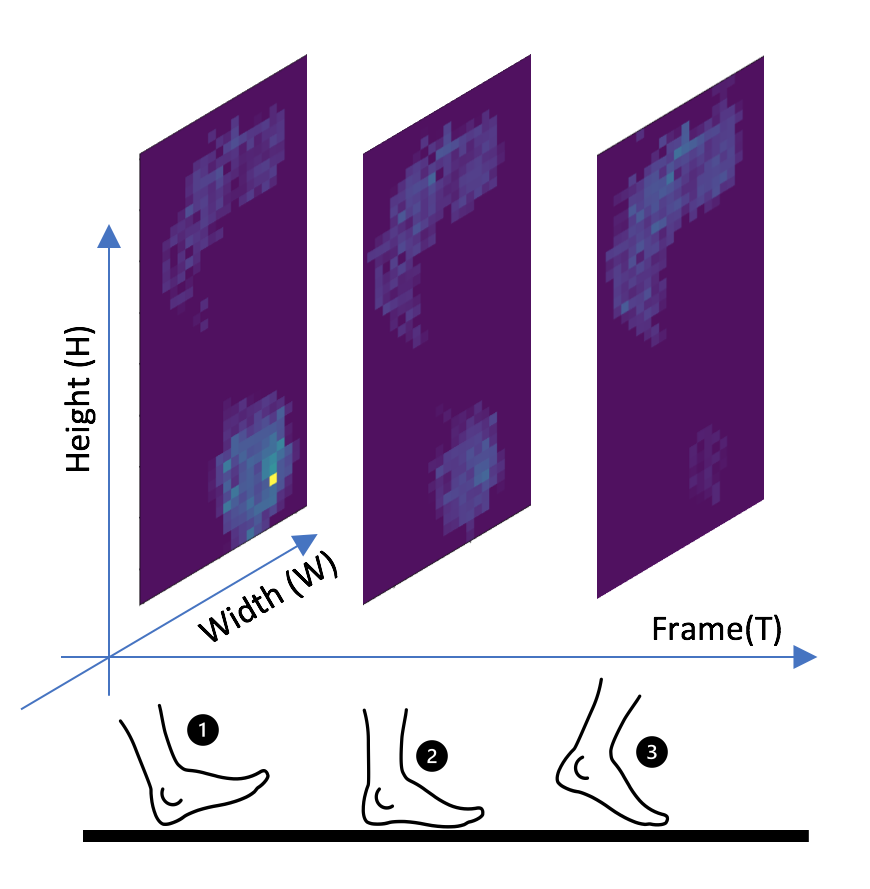
\includegraphics[width=\textwidth]{figures/project/frame2.png}
    \end{minipage}
    \caption{Different frames of footprint video in Stepscan dataset.}
    \label{fig:Stepscan_dataset}
\end{figure}

%%************
In general, there are two modes for footprint recognition or generally in the biometric system: verification or identification mode \cite{Jain2004AnRecognition}. In verification mode, the biometric system is used for accessing buildings or data. In other words, the system compares the claimed person with its dataset to determine whether or not the claim is valid. These systems not only consume less processing power and time but also have better performance regarding identification systems \cite{Jain2004AnRecognition}. Moreover, verification systems could be implemented on a small scale. This project aims to find some features from the datasets to construct a classifier for verification purposes. 

%Because verification systems only need to compare the presented biometric to a biometric reference stored in the system, they can generate results more quickly and are more accurate than identification systems, even when the size of the database increases.


The rest of this paper is organized as follows: Section 2 provides the relevant works and researches. Then, the classification method based on machine learning and deep learning is presented in Section 3. The results and discussion are described in Sections 4 and 5.

%%$$The rest of this paper is organized as follows: Section 2 provides the relevant works and researches. Then, the classification method based on machine learning and deep learning is presented in Section 3. Also a brief survey on time series classification and Deep learning is provided in \ref{appendix:2}. The results and discussion are described in Sections 4 and 5.

% in Section 3, the time domain features as well as machine learning models are defined. In Section 4, we discuss the results, and we propose future work in Section 5.



Furthermore, this research will be implemented in Python, and the source codes are available on the GitHub repository \cite{SKazemii/EE6563}. 









